\subsection{Prediction Model} \label{subsec:prediction-model}

Consecutive feature frames from the \nameref{subsec:feature-extraction} module
are concatenated in order to form a \emph{segment}. This segment is then fed to
the prediction model. Which will output a motion estimation.

This work proposes a shallow Convolutional Neural Network \cite{FukushimaCNN}
composed by two convolution layers, each of them followed by a max pooling
layer, and two fully connected layers, each of them preceded by a dropout, as
shown in \cref{fig:model-arch-cnn}. 


% TODO Could save space by adding numbers to the figure
\begin{figure}
    \centering
    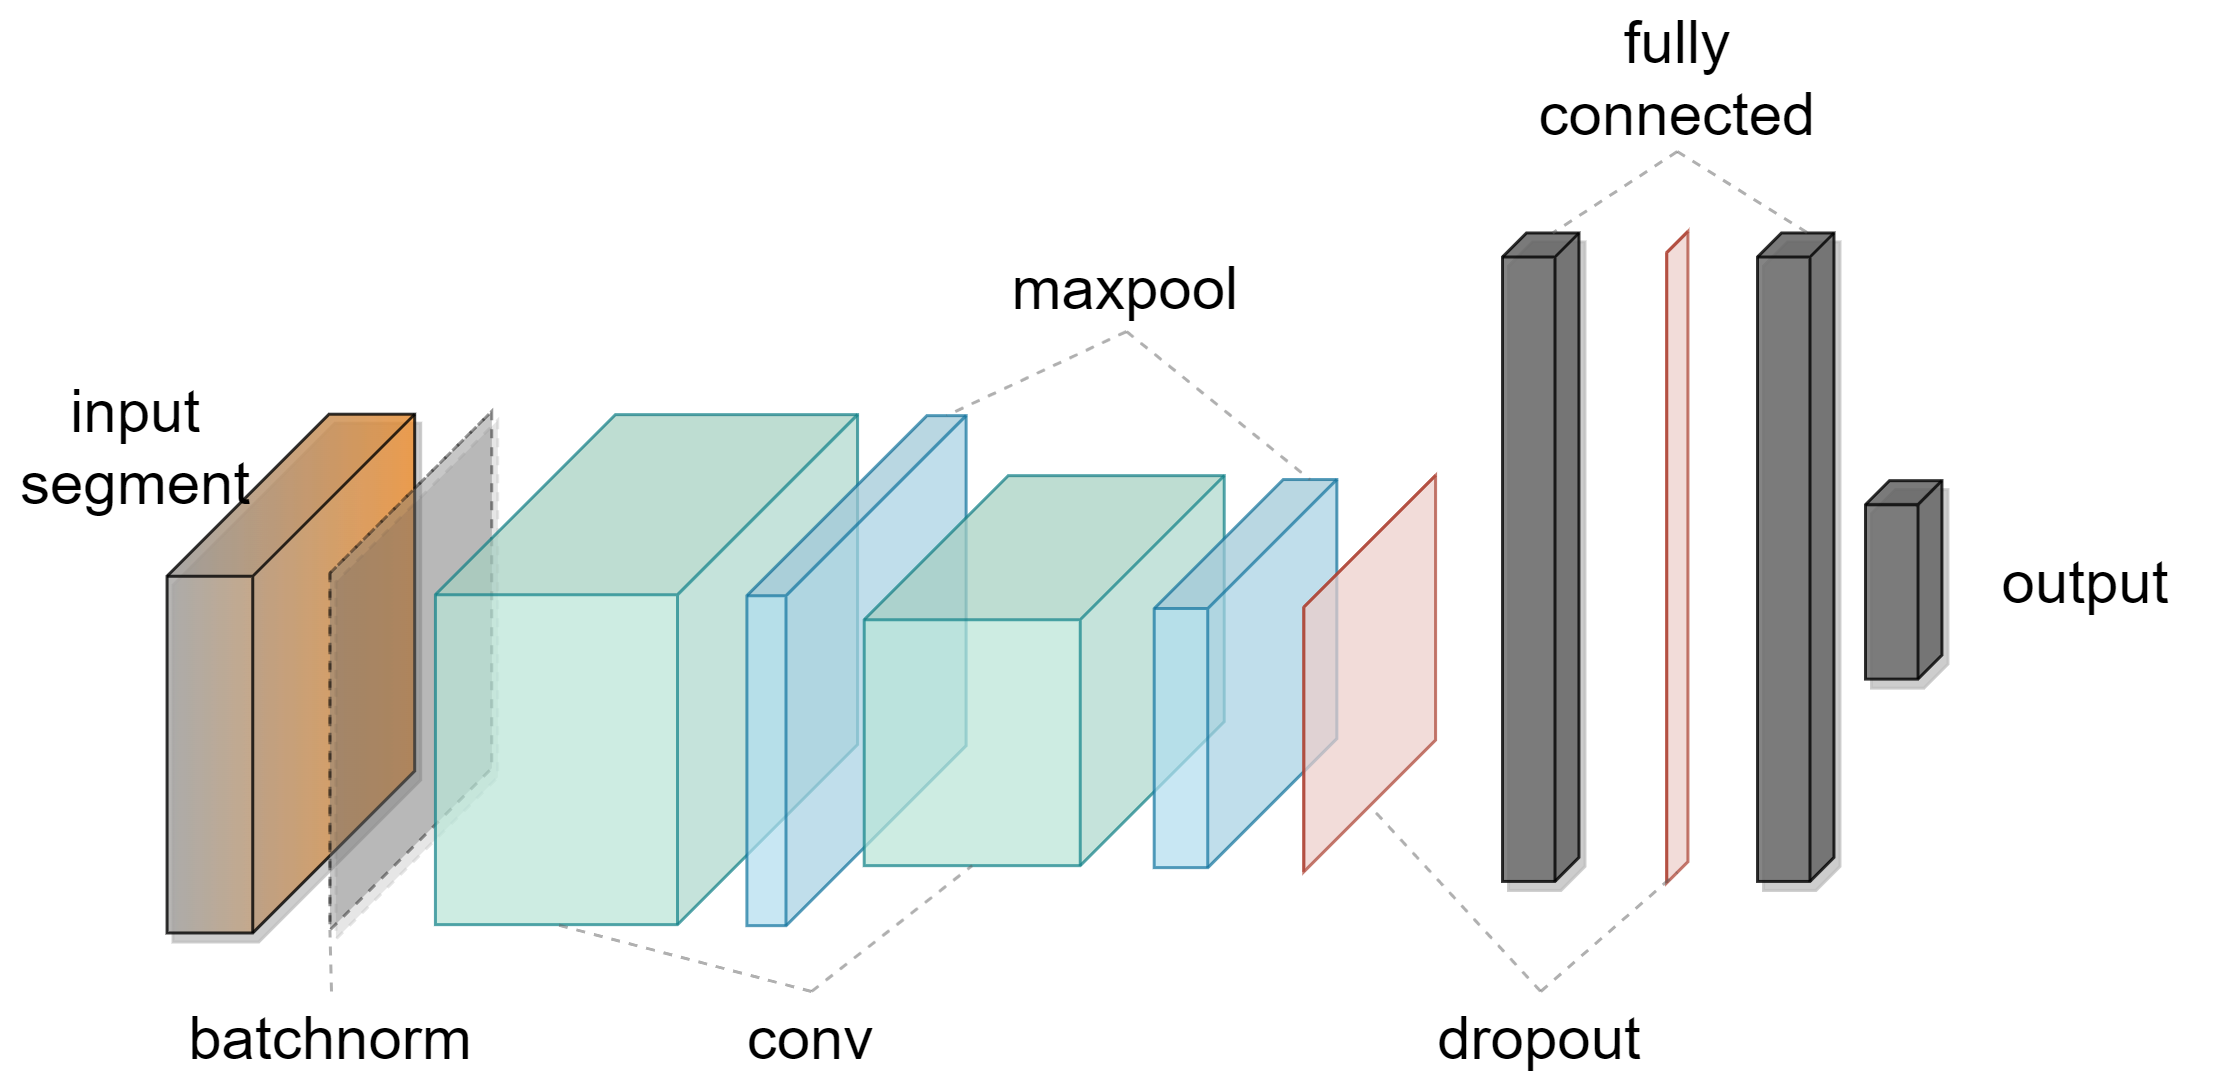
\includegraphics[width=\linewidth]{\subdir/CNN.drawio.png}
    \caption{Shallow Convolutional Neural Network architecture proposed in this
    work. The selected model is composed by: a batch normalization layer; a
    first convolution layer with one input channel, a kernel size of 5 and 16
    output channels; a second convolution layer with 32 output channels and a
    kernel size of 2; a first fully connected layer with an output size of 256;
    a second fully connected layer with an output size of 28. Each of the
    convolution layers is followed by a maxpool layer with a kernel size of 2
    and each of the fully connected layers is preceded by a dropout layer with
    a probability of 50\%.}
    \label{fig:model-arch-cnn}
\end{figure}

The input dimensions depend on the \nameref{subsec:feature-extraction}
parameters, namely number of features per frame, number of extractors and
number of frames per segment. Layer sizes and the output of the last fully
connected layers are seen as tuneable parameters as well. Experiments are
conducted with the different parameters and a model is selected based on its
performance and computational cost.

% \subsubsection{Task} \label{subsec:model-task}

% One can find here a description of the different tasks implemented and tested
% in models. Tasks define the goal of the model and the way its loss is computed.

% \paragraph{Classification} \label{para:model-task-class} Consists in
% classifying the longitudinal velocity given a set of possibilities. The
% different classes are ranges of longitudinal velocities, being these ranges a
% hyperparameter of the model. Cross entropy loss is computed between the
% predicted class probabilities and the class corresponding to the target
% longitudinal velocity and the predicted class. The output of the model is
% therefore a vector of probabilities corresponding to each class.

% \paragraph{Ordinal classification} \label{para:model-task-ord-class} Consists
% in classifying the longitudinal velocity given a set of possibilities like in
% \nameref{para:model-task-class}, with different classes being ranges of
% longitudinal velocities. But the order of the class matters. This method was
% introduced in \cite{ordclass2006}, where standard classification algorithms are
% extended to make use of the order of the classes. The output of this model is a
% vector of binary values that can be decoded into a class position by making use
% of a ranking rule. The loss is computed with the mean square error between the
% target class position and the predicted class position. 

% \subsubsection{Architecture} \label{subsec:model-architecture}

% This section describes the different model architectures implemented and
% evaluated. A common point of them all is simplicity. It is out of the scope of
% this work to find an optimal architecture for acoustic odometry. But it is
% interesting to evaluate different simple options.

% \paragraph{CNN with normalized input} \label{para:model-arch-norm-cnn} This
% architecture is identical to the \nameref{para:model-arch-cnn} except for the
% fact that it contains a batch normalization layer \cite{batchnorm2015} as shown
% in \cref{fig:model-arch-cnn}.